% Options for packages loaded elsewhere
\PassOptionsToPackage{unicode}{hyperref}
\PassOptionsToPackage{hyphens}{url}
%
\documentclass[
]{article}
\usepackage{amsmath,amssymb}
\usepackage{lmodern}
\usepackage{iftex}
\ifPDFTeX
  \usepackage[T1]{fontenc}
  \usepackage[utf8]{inputenc}
  \usepackage{textcomp} % provide euro and other symbols
\else % if luatex or xetex
  \usepackage{unicode-math}
  \defaultfontfeatures{Scale=MatchLowercase}
  \defaultfontfeatures[\rmfamily]{Ligatures=TeX,Scale=1}
\fi
% Use upquote if available, for straight quotes in verbatim environments
\IfFileExists{upquote.sty}{\usepackage{upquote}}{}
\IfFileExists{microtype.sty}{% use microtype if available
  \usepackage[]{microtype}
  \UseMicrotypeSet[protrusion]{basicmath} % disable protrusion for tt fonts
}{}
\makeatletter
\@ifundefined{KOMAClassName}{% if non-KOMA class
  \IfFileExists{parskip.sty}{%
    \usepackage{parskip}
  }{% else
    \setlength{\parindent}{0pt}
    \setlength{\parskip}{6pt plus 2pt minus 1pt}}
}{% if KOMA class
  \KOMAoptions{parskip=half}}
\makeatother
\usepackage{xcolor}
\usepackage[margin=1in]{geometry}
\usepackage{color}
\usepackage{fancyvrb}
\newcommand{\VerbBar}{|}
\newcommand{\VERB}{\Verb[commandchars=\\\{\}]}
\DefineVerbatimEnvironment{Highlighting}{Verbatim}{commandchars=\\\{\}}
% Add ',fontsize=\small' for more characters per line
\usepackage{framed}
\definecolor{shadecolor}{RGB}{248,248,248}
\newenvironment{Shaded}{\begin{snugshade}}{\end{snugshade}}
\newcommand{\AlertTok}[1]{\textcolor[rgb]{0.94,0.16,0.16}{#1}}
\newcommand{\AnnotationTok}[1]{\textcolor[rgb]{0.56,0.35,0.01}{\textbf{\textit{#1}}}}
\newcommand{\AttributeTok}[1]{\textcolor[rgb]{0.77,0.63,0.00}{#1}}
\newcommand{\BaseNTok}[1]{\textcolor[rgb]{0.00,0.00,0.81}{#1}}
\newcommand{\BuiltInTok}[1]{#1}
\newcommand{\CharTok}[1]{\textcolor[rgb]{0.31,0.60,0.02}{#1}}
\newcommand{\CommentTok}[1]{\textcolor[rgb]{0.56,0.35,0.01}{\textit{#1}}}
\newcommand{\CommentVarTok}[1]{\textcolor[rgb]{0.56,0.35,0.01}{\textbf{\textit{#1}}}}
\newcommand{\ConstantTok}[1]{\textcolor[rgb]{0.00,0.00,0.00}{#1}}
\newcommand{\ControlFlowTok}[1]{\textcolor[rgb]{0.13,0.29,0.53}{\textbf{#1}}}
\newcommand{\DataTypeTok}[1]{\textcolor[rgb]{0.13,0.29,0.53}{#1}}
\newcommand{\DecValTok}[1]{\textcolor[rgb]{0.00,0.00,0.81}{#1}}
\newcommand{\DocumentationTok}[1]{\textcolor[rgb]{0.56,0.35,0.01}{\textbf{\textit{#1}}}}
\newcommand{\ErrorTok}[1]{\textcolor[rgb]{0.64,0.00,0.00}{\textbf{#1}}}
\newcommand{\ExtensionTok}[1]{#1}
\newcommand{\FloatTok}[1]{\textcolor[rgb]{0.00,0.00,0.81}{#1}}
\newcommand{\FunctionTok}[1]{\textcolor[rgb]{0.00,0.00,0.00}{#1}}
\newcommand{\ImportTok}[1]{#1}
\newcommand{\InformationTok}[1]{\textcolor[rgb]{0.56,0.35,0.01}{\textbf{\textit{#1}}}}
\newcommand{\KeywordTok}[1]{\textcolor[rgb]{0.13,0.29,0.53}{\textbf{#1}}}
\newcommand{\NormalTok}[1]{#1}
\newcommand{\OperatorTok}[1]{\textcolor[rgb]{0.81,0.36,0.00}{\textbf{#1}}}
\newcommand{\OtherTok}[1]{\textcolor[rgb]{0.56,0.35,0.01}{#1}}
\newcommand{\PreprocessorTok}[1]{\textcolor[rgb]{0.56,0.35,0.01}{\textit{#1}}}
\newcommand{\RegionMarkerTok}[1]{#1}
\newcommand{\SpecialCharTok}[1]{\textcolor[rgb]{0.00,0.00,0.00}{#1}}
\newcommand{\SpecialStringTok}[1]{\textcolor[rgb]{0.31,0.60,0.02}{#1}}
\newcommand{\StringTok}[1]{\textcolor[rgb]{0.31,0.60,0.02}{#1}}
\newcommand{\VariableTok}[1]{\textcolor[rgb]{0.00,0.00,0.00}{#1}}
\newcommand{\VerbatimStringTok}[1]{\textcolor[rgb]{0.31,0.60,0.02}{#1}}
\newcommand{\WarningTok}[1]{\textcolor[rgb]{0.56,0.35,0.01}{\textbf{\textit{#1}}}}
\usepackage{graphicx}
\makeatletter
\def\maxwidth{\ifdim\Gin@nat@width>\linewidth\linewidth\else\Gin@nat@width\fi}
\def\maxheight{\ifdim\Gin@nat@height>\textheight\textheight\else\Gin@nat@height\fi}
\makeatother
% Scale images if necessary, so that they will not overflow the page
% margins by default, and it is still possible to overwrite the defaults
% using explicit options in \includegraphics[width, height, ...]{}
\setkeys{Gin}{width=\maxwidth,height=\maxheight,keepaspectratio}
% Set default figure placement to htbp
\makeatletter
\def\fps@figure{htbp}
\makeatother
\setlength{\emergencystretch}{3em} % prevent overfull lines
\providecommand{\tightlist}{%
  \setlength{\itemsep}{0pt}\setlength{\parskip}{0pt}}
\setcounter{secnumdepth}{-\maxdimen} % remove section numbering
\ifLuaTeX
  \usepackage{selnolig}  % disable illegal ligatures
\fi
\IfFileExists{bookmark.sty}{\usepackage{bookmark}}{\usepackage{hyperref}}
\IfFileExists{xurl.sty}{\usepackage{xurl}}{} % add URL line breaks if available
\urlstyle{same} % disable monospaced font for URLs
\hypersetup{
  pdftitle={BIOMI6300\_Project1:OMV\_Analysis},
  pdfauthor={Jiucheng Ding},
  hidelinks,
  pdfcreator={LaTeX via pandoc}}

\title{BIOMI6300\_Project1:OMV\_Analysis}
\author{Jiucheng Ding}
\date{2023-02-23}

\begin{document}
\maketitle

\#File setup:

\begin{Shaded}
\begin{Highlighting}[]
\NormalTok{knitr}\SpecialCharTok{::}\NormalTok{opts\_chunk}\SpecialCharTok{$}\FunctionTok{set}\NormalTok{(}\AttributeTok{echo =} \ConstantTok{TRUE}\NormalTok{)}
\end{Highlighting}
\end{Shaded}

\#Adding Introduction: Outer membrane vesicles (OMVs) are derived from
Gram-negative bacteria, are formed through a budding and release
mechanism on the outer membrane. The spheres are ranged between 20-200
nm in diameter, encapsulated mostly by lipids.They contain bioactive
proteins and other components and thus may play biological roles to the
neighboring microbiome community and to the host. Although the
production of OMVs have been well-reported and documented, the mechanism
behind is still not quite clear; investigation on their formation
mechanisms and bioactive roles is still required. This study tracked the
growth and vesiculation values of the whole genome knockout library of
Escherichia coli mutant strains through a high-throughput experimental
method and systems-scale analysis. The mutations were reported to
truncate the structure of the OMVs and led to hypervesiculation, and
mutants in oxidative stress perform lowered level of vesiculation in
E.coli.

\#Install tidyverse without installation message:

\begin{Shaded}
\begin{Highlighting}[]
\FunctionTok{library}\NormalTok{(tidyverse)}
\end{Highlighting}
\end{Shaded}

\begin{verbatim}
## -- Attaching packages --------------------------------------- tidyverse 1.3.2 --
## v ggplot2 3.4.0     v purrr   1.0.1
## v tibble  3.1.8     v dplyr   1.1.0
## v tidyr   1.3.0     v stringr 1.5.0
## v readr   2.1.3     v forcats 1.0.0
## -- Conflicts ------------------------------------------ tidyverse_conflicts() --
## x dplyr::filter() masks stats::filter()
## x dplyr::lag()    masks stats::lag()
\end{verbatim}

\#Loading data of OMV production values:

\begin{Shaded}
\begin{Highlighting}[]
\NormalTok{vesiculation}\OtherTok{\textless{}{-}} \FunctionTok{read\_csv}\NormalTok{(}\StringTok{"../Data/vesiculation.csv"}\NormalTok{)}
\end{Highlighting}
\end{Shaded}

\begin{verbatim}
## Rows: 3908 Columns: 16
## -- Column specification --------------------------------------------------------
## Delimiter: ","
## chr  (2): CommonName, bID
## dbl (14): GenBankID, OMV.Trial1, OMV.Trial2, OMV.Trial3, OMV.Trial4, OMV.Tri...
## 
## i Use `spec()` to retrieve the full column specification for this data.
## i Specify the column types or set `show_col_types = FALSE` to quiet this message.
\end{verbatim}

\#Perfrom some analysis with this OMV production data: \#The data file
shows the difference in OMV production of the gene-knockout library
comparing to their normal state.

\begin{Shaded}
\begin{Highlighting}[]
\FunctionTok{summarize}\NormalTok{(vesiculation, }
          \AttributeTok{averageLogOMV=}\FunctionTok{mean}\NormalTok{(average.log.OMV), }
          \AttributeTok{minimumLogOMV=}\FunctionTok{min}\NormalTok{(average.log.OMV),}
          \AttributeTok{maximumLogOMV=}\FunctionTok{max}\NormalTok{(average.log.OMV),}
          \AttributeTok{medianLogOMV=}\FunctionTok{median}\NormalTok{(average.log.OMV),}
          \AttributeTok{stdevLogOMV=}\FunctionTok{sd}\NormalTok{(average.log.OMV),}
          
          \AttributeTok{averageAntilogOMV=}\FunctionTok{mean}\NormalTok{(average.antilog.omv),}
          \AttributeTok{minimumAntilogOMV=}\FunctionTok{min}\NormalTok{(average.antilog.omv),}
          \AttributeTok{maximumAntilogOMV=}\FunctionTok{max}\NormalTok{(average.antilog.omv),}
          \AttributeTok{medianAntilogOMV=}\FunctionTok{median}\NormalTok{(average.antilog.omv),}
          
          \AttributeTok{averageSTDEVAntilog=}\FunctionTok{mean}\NormalTok{(stdev.antilog))}
\end{Highlighting}
\end{Shaded}

\begin{verbatim}
## # A tibble: 1 x 10
##   averageLogOMV minim~1 maxim~2 median~3 stdev~4 avera~5 minim~6 maxim~7 media~8
##           <dbl>   <dbl>   <dbl>    <dbl>   <dbl>   <dbl>   <dbl>   <dbl>   <dbl>
## 1       -0.0255   -1.49    1.34 -0.00174   0.212    1.09  0.0351    24.2    1.02
## # ... with 1 more variable: averageSTDEVAntilog <dbl>, and abbreviated variable
## #   names 1: minimumLogOMV, 2: maximumLogOMV, 3: medianLogOMV, 4: stdevLogOMV,
## #   5: averageAntilogOMV, 6: minimumAntilogOMV, 7: maximumAntilogOMV,
## #   8: medianAntilogOMV
\end{verbatim}

\#Then make scatterplot to show the distribution of OMV production
change (linear) for all samples, with a few outliers removed.

\begin{Shaded}
\begin{Highlighting}[]
\FunctionTok{ggplot}\NormalTok{(}\AttributeTok{data=}\NormalTok{vesiculation) }\SpecialCharTok{+}
  \FunctionTok{aes}\NormalTok{(}\AttributeTok{x=}\NormalTok{bID) }\SpecialCharTok{+} 
  \FunctionTok{labs}\NormalTok{(}\AttributeTok{x=} \StringTok{"E.coli K12 unique identifier"}\NormalTok{) }\SpecialCharTok{+}
  \FunctionTok{aes}\NormalTok{(}\AttributeTok{y=}\NormalTok{average.antilog.omv) }\SpecialCharTok{+}
  \FunctionTok{ylim}\NormalTok{(}\SpecialCharTok{{-}}\DecValTok{1}\NormalTok{,}\DecValTok{8}\NormalTok{)}\SpecialCharTok{+}
  \FunctionTok{labs}\NormalTok{(}\AttributeTok{y=}\StringTok{"Average OMV Production Change (Folds)"}\NormalTok{)}\SpecialCharTok{+}
  \FunctionTok{geom\_point}\NormalTok{(}\AttributeTok{size=}\FloatTok{0.20}\NormalTok{,}\AttributeTok{alpha=}\FloatTok{0.6}\NormalTok{)}\SpecialCharTok{+}
  \FunctionTok{geom\_hline}\NormalTok{(}\AttributeTok{yintercept=}\DecValTok{1}\NormalTok{, }\AttributeTok{color=}\StringTok{"blue"}\NormalTok{, }\AttributeTok{linetype=}\StringTok{"solid"}\NormalTok{, }\AttributeTok{size=}\DecValTok{1}\NormalTok{)}\SpecialCharTok{+}
  \FunctionTok{geom\_hline}\NormalTok{(}\AttributeTok{yintercept=}\FloatTok{1.091811}\NormalTok{, }\AttributeTok{color=}\StringTok{"orange"}\NormalTok{,}\AttributeTok{linetype=}\StringTok{"dashed"}\NormalTok{, }\AttributeTok{size=}\FloatTok{0.7}\NormalTok{)}
\end{Highlighting}
\end{Shaded}

\begin{verbatim}
## Warning: Using `size` aesthetic for lines was deprecated in ggplot2 3.4.0.
## i Please use `linewidth` instead.
\end{verbatim}

\begin{verbatim}
## Warning: Removed 2 rows containing missing values (`geom_point()`).
\end{verbatim}

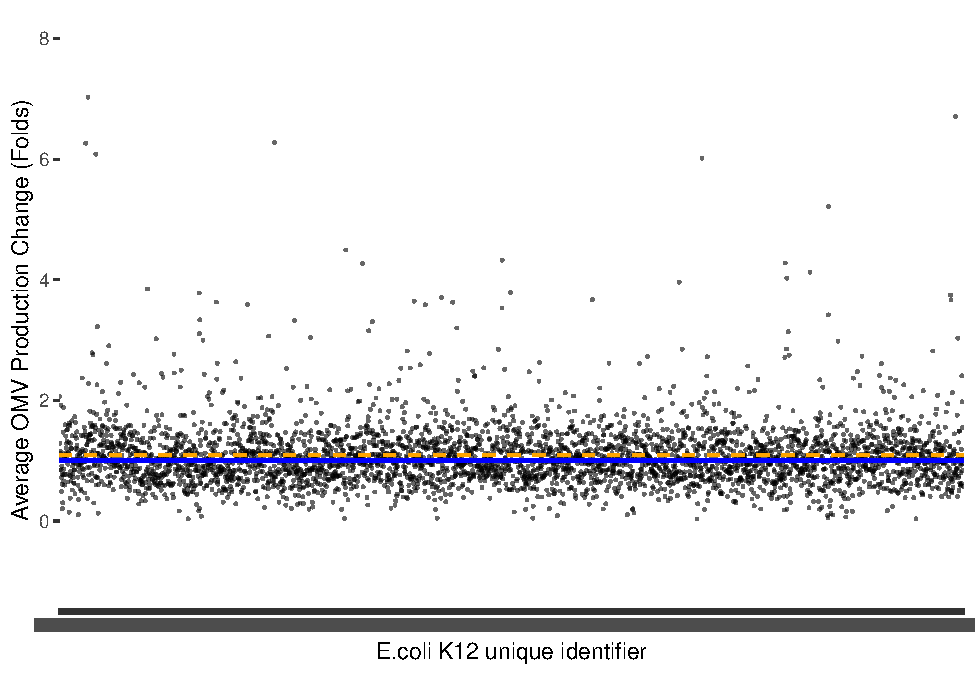
\includegraphics{OMV-analysis_files/figure-latex/figure1-1.pdf}

\begin{Shaded}
\begin{Highlighting}[]
  \FunctionTok{labs}\NormalTok{(}\AttributeTok{title =} \StringTok{"Average impact on OMV production (Antilogged, Linear)"}\NormalTok{)}
\end{Highlighting}
\end{Shaded}

\begin{verbatim}
## $title
## [1] "Average impact on OMV production (Antilogged, Linear)"
## 
## attr(,"class")
## [1] "labels"
\end{verbatim}

Figure1: This scatterplot shows the OMV production change in antilog,
linear. Each dot represents an individual sample.A few outliers above 8
folds are ignored. The blue solid has a y-intercept of 1, indicating
that the values above this line have an increased OMV production; those
below represent those with lowered OMV production.

\#Let's make another figure with same data, but in log10 scale.

\begin{Shaded}
\begin{Highlighting}[]
\FunctionTok{ggplot}\NormalTok{(}\AttributeTok{data=}\NormalTok{vesiculation) }\SpecialCharTok{+}
  \FunctionTok{aes}\NormalTok{(}\AttributeTok{x=}\NormalTok{bID) }\SpecialCharTok{+} 
  \FunctionTok{labs}\NormalTok{(}\AttributeTok{x=} \StringTok{"E.coli K12 unique identifier"}\NormalTok{) }\SpecialCharTok{+}
  \FunctionTok{aes}\NormalTok{(}\AttributeTok{y=}\NormalTok{average.log.OMV) }\SpecialCharTok{+}
  \FunctionTok{labs}\NormalTok{(}\AttributeTok{y=}\StringTok{"Average OMV Production Change (log10 of Folds)"}\NormalTok{)}\SpecialCharTok{+}
  \FunctionTok{geom\_point}\NormalTok{(}\AttributeTok{size=}\FloatTok{0.25}\NormalTok{, }\AttributeTok{alpha=}\FloatTok{0.6}\NormalTok{)}\SpecialCharTok{+}
  \FunctionTok{geom\_hline}\NormalTok{(}\AttributeTok{yintercept=}\DecValTok{0}\NormalTok{, }\AttributeTok{color=}\StringTok{"blue"}\NormalTok{, }\AttributeTok{linetype=}\StringTok{"solid"}\NormalTok{, }\AttributeTok{size=}\DecValTok{1}\NormalTok{)}\SpecialCharTok{+}
  \FunctionTok{geom\_hline}\NormalTok{(}\AttributeTok{yintercept=}\SpecialCharTok{{-}}\FloatTok{0.02552768}\NormalTok{, }\AttributeTok{color=}\StringTok{"orange"}\NormalTok{,}\AttributeTok{linetype=}\StringTok{"dashed"}\NormalTok{, }\AttributeTok{size=}\FloatTok{0.7}\NormalTok{)}
\end{Highlighting}
\end{Shaded}

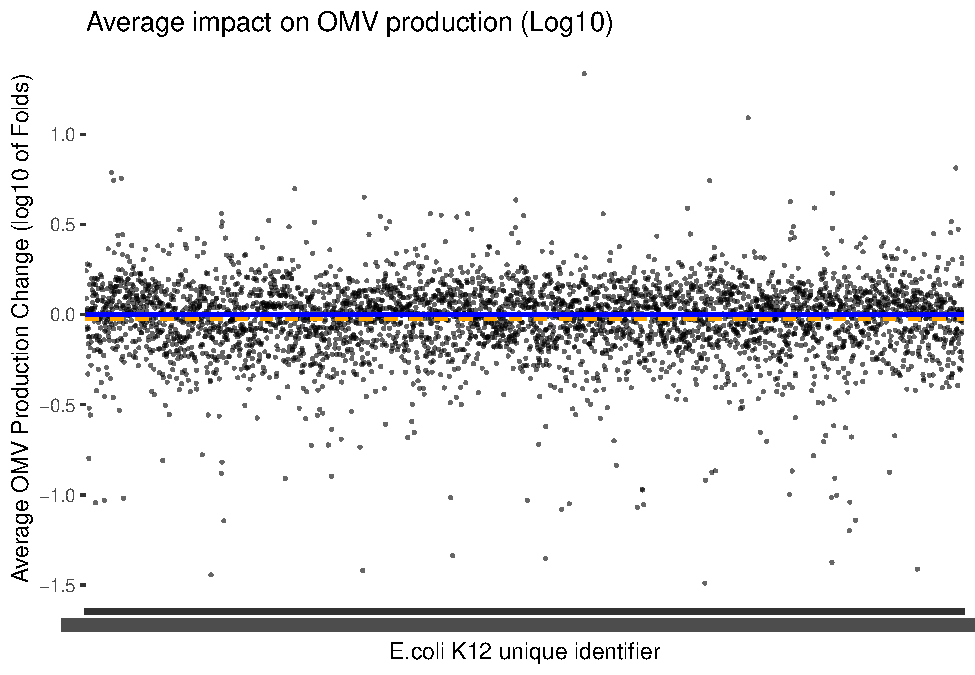
\includegraphics{OMV-analysis_files/figure-latex/figure2-1.pdf}

\begin{Shaded}
\begin{Highlighting}[]
  \FunctionTok{labs}\NormalTok{(}\AttributeTok{title =} \StringTok{"Average impact on OMV production (Log10)"}\NormalTok{)}
\end{Highlighting}
\end{Shaded}

\begin{verbatim}
## $title
## [1] "Average impact on OMV production (Log10)"
## 
## attr(,"class")
## [1] "labels"
\end{verbatim}

Figure2:This scatterplot shows the OMV production change in log10. Each
dot represents an individual sample.The blue solid has a y-intercept of
0, indicating that the values above this line have an increased OMV
production; those below represent those with lowered OMV production
level.

\#Make a histogram showing the frequency.

\begin{Shaded}
\begin{Highlighting}[]
\FunctionTok{ggplot}\NormalTok{(}\AttributeTok{data=}\NormalTok{vesiculation) }\SpecialCharTok{+}
  \FunctionTok{aes}\NormalTok{(}\AttributeTok{x=}\NormalTok{average.log.OMV) }\SpecialCharTok{+}
  \FunctionTok{labs}\NormalTok{(}\AttributeTok{x=}\StringTok{"Change on OMV production, log10"}\NormalTok{) }\SpecialCharTok{+}
  \FunctionTok{aes}\NormalTok{(}\AttributeTok{y=}\NormalTok{..count..) }\SpecialCharTok{+}
  \FunctionTok{labs}\NormalTok{(}\AttributeTok{y=}\StringTok{"Frequency"}\NormalTok{) }\SpecialCharTok{+}
  \FunctionTok{scale\_y\_continuous}\NormalTok{(}\AttributeTok{breaks =} \FunctionTok{seq}\NormalTok{(}\DecValTok{0}\NormalTok{, }\DecValTok{140}\NormalTok{, }\AttributeTok{by =} \DecValTok{20}\NormalTok{))}\SpecialCharTok{+}
  \FunctionTok{geom\_histogram}\NormalTok{(}\AttributeTok{color=}\StringTok{"black"}\NormalTok{,}\AttributeTok{binwidth=}\FloatTok{0.01}\NormalTok{) }\SpecialCharTok{+}
  \FunctionTok{geom\_vline}\NormalTok{(}\FunctionTok{aes}\NormalTok{(}\AttributeTok{xintercept=}\DecValTok{0}\NormalTok{, }\AttributeTok{color=}\StringTok{"No Change in OMV"}\NormalTok{), }\AttributeTok{size=}\FloatTok{0.7}\NormalTok{, }\AttributeTok{linetype=}\StringTok{"solid"}\NormalTok{) }\SpecialCharTok{+}
  \FunctionTok{geom\_vline}\NormalTok{(}\FunctionTok{aes}\NormalTok{(}\AttributeTok{xintercept=}\FunctionTok{mean}\NormalTok{(vesiculation}\SpecialCharTok{$}\NormalTok{average.log.OMV), }\AttributeTok{color=}\StringTok{"Mean"}\NormalTok{), }\AttributeTok{size=}\FloatTok{0.7}\NormalTok{, }\AttributeTok{linetype=}\StringTok{"dashed"}\NormalTok{) }\SpecialCharTok{+}
  \FunctionTok{scale\_color\_manual}\NormalTok{(}\AttributeTok{values=}\FunctionTok{c}\NormalTok{(}\StringTok{"No Change in OMV"}\OtherTok{=}\StringTok{"blue"}\NormalTok{, }\StringTok{"Mean"}\OtherTok{=}\StringTok{"orange"}\NormalTok{)) }\SpecialCharTok{+}
  \FunctionTok{labs}\NormalTok{(}\AttributeTok{title=}\StringTok{"Distribution of OMV production in log10"}\NormalTok{, }\AttributeTok{color=}\StringTok{""}\NormalTok{) }
\end{Highlighting}
\end{Shaded}

\begin{verbatim}
## Warning: The dot-dot notation (`..count..`) was deprecated in ggplot2 3.4.0.
## i Please use `after_stat(count)` instead.
\end{verbatim}

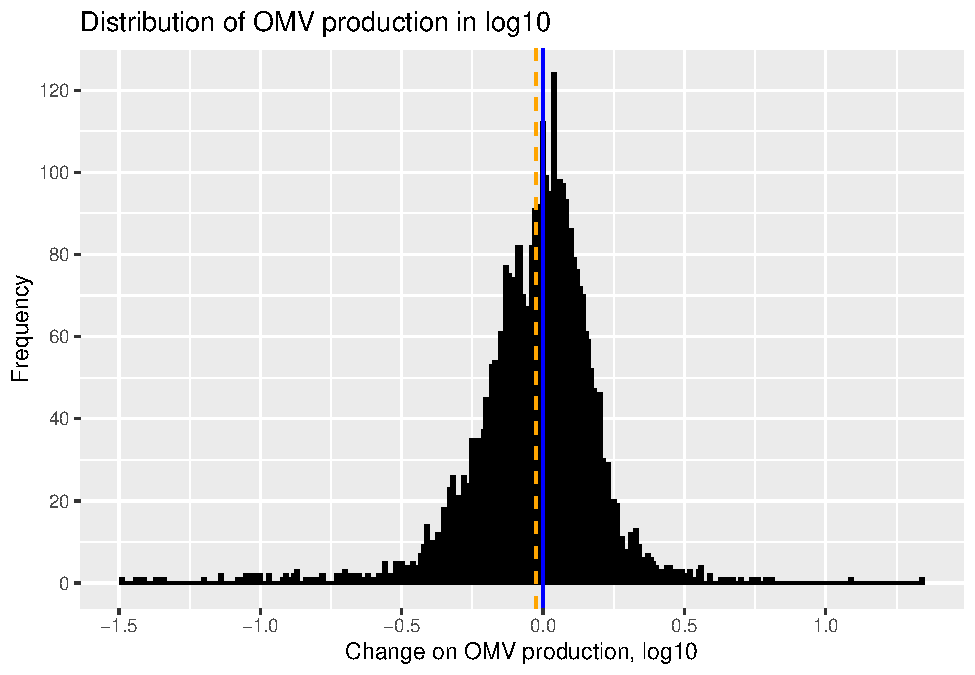
\includegraphics{OMV-analysis_files/figure-latex/figure3-1.pdf}
Figure3:Histogram for the distribution of change on OMV production
relative to the normal state of E.coli. In log 10. The blue dashed line
shows when change on OMV production is 0, meaning there is no change.

\#To determine the session info: install.packages(``devtools'')
library(devtools) session\_info()

\end{document}
